\section{Nucleon-Nucleon Interaction}%
\label{sec:nucleon_nucleon_interaction}

Due to the lack of a exact theory to describe the nucleon-nucleon (\gls{NN}) interaction, a model need to be imposed and fit with experimental measurement or theoretical calculation results. Plus, for a system as massive as a \gls{NS}, deducing the \gls{EoS} using the \emph{ab initio} method, i.e. solving the Schr\"{o}dinger equation over all particles, is simply impossible, therefore an \emph{effective interaction} must be used \citep{greiner1996nuclear}. In this section, we only limit ourselves to two-body interaction, thus, the \gls{NN} potential can be expressed in the form of
\begin{equation}
        v = v(\bm{r}, \bm{r'}, \bm{p}, \bm{p'}, \bm{\sigma}, \bm{\sigma'}, \bm{\tau}, \bm{\tau'})
        \label{eff_interaction}
\end{equation}
where the primed and unprimed variables indicate the properties of 2 nucleons respectively, in which $\bm{r}$ is the particle's position, $\bm{p}$ is its momentum, $\bm{\sigma}$ is its intrinsic spin and $\bm{\tau}$ is its isospin.\par
The functional form of $v$ in \eqref{eff_interaction} cannot freely take any form but is constrained by many invariance requirements \citep{greiner1996nuclear}, namely the translational, Galilei, rotational, isospin, parity and time reversal invariance. Having such considerations, developing further the M3Y-Paris interaction, which was used by the \gls{HF} study of \gls{NM} \citep{loan2011equation, tan2016mean, tan2020spin,tan2021equation} and the folding model study of \gls{NN} scattering \citep{khoa1997nuclear,khoa2000generalized},
\begin{equation}
        v = v_{00}(r) + v_{10}(r) \bm{\sigma}\cdot\bm{\sigma'} + v_{01}(r) \bm{\tau}\cdot\bm{\tau'} + v_{11}(r) (\bm{\sigma}\cdot\bm{\sigma'})(\bm{\tau}\cdot\bm{\tau'})
\end{equation}
by adding a density-dependent form factor $F_{\sigma\tau}(n)$ to each term gives the CDM3Y$n$ and BDM3Y1 interaction model
\begin{IEEEeqnarray*}{rCl}
        v(n,r) &=& F_{00}(n) v_{00}(r) + F_{10}(n) v_{10}(r) \bm{\sigma}\cdot\bm{\sigma'}\\
          &&\negmedspace{}+ F_{01}(n) v_{01}(r) \bm{\tau}\cdot\bm{\tau'} + F_{11}(n) v_{11}(r) (\bm{\sigma}\cdot\bm{\sigma'})(\bm{\tau}\cdot\bm{\tau'})\IEEEyesnumber
          \label{eq2-11}
\end{IEEEeqnarray*}  
where each radial term is the superposition of 3 Yukawa potentials
\begin{equation}
        v_{\sigma\tau}(r) = \sum^{3}_{k=1} Y_{\sigma\tau}(k) \frac{\exp(-\mu_k r)}{\mu_k r} 
\end{equation}
and the form factor $F_{\sigma\tau}(n)$ shared the functional form \citep{khoa1997nuclear,tan2020spin,tan2021equation,than2010ufr}
\begin{equation}
        F_{\sigma\tau}(n) = C_{\sigma\tau} [1 + \alpha_{\sigma\tau} \exp(-\beta_{\sigma\tau}n) + \gamma_{\sigma\tau}n]
\end{equation}
with parameters given in Table \ref{tab:cd}. The parameters of $F_{00}$ were adjusted to give the corresponding values of incompressibility $K$ of symmetric \gls{NM} at saturation density $n_0$ and the binding energy $E_0 \approx 15.8\; MeV$, while the 10 term is modified from \citep{than2010ufr} to reproduce $E_{sym}(n_0) \approx 30\;MeV$, $L\approx 50\;MeV$ and to be in agreement with the ab-initio results \citep{akmal1998equation,gandolfi2010microscopic} at higher density \citep{tan2021equation}. On the other hand, the spin-dependent terms, 10 and 11, are hereby included in the 5 models by fine tuning the parameters to yield the same result as the Brueckner-Hartree-Fock (\gls{BHF}) study of spin polarized \gls{NM} \citep{vidana2002equation} as in Figure \ref{fig:bhf}.

\begin{figure}[ht]
        \centering
        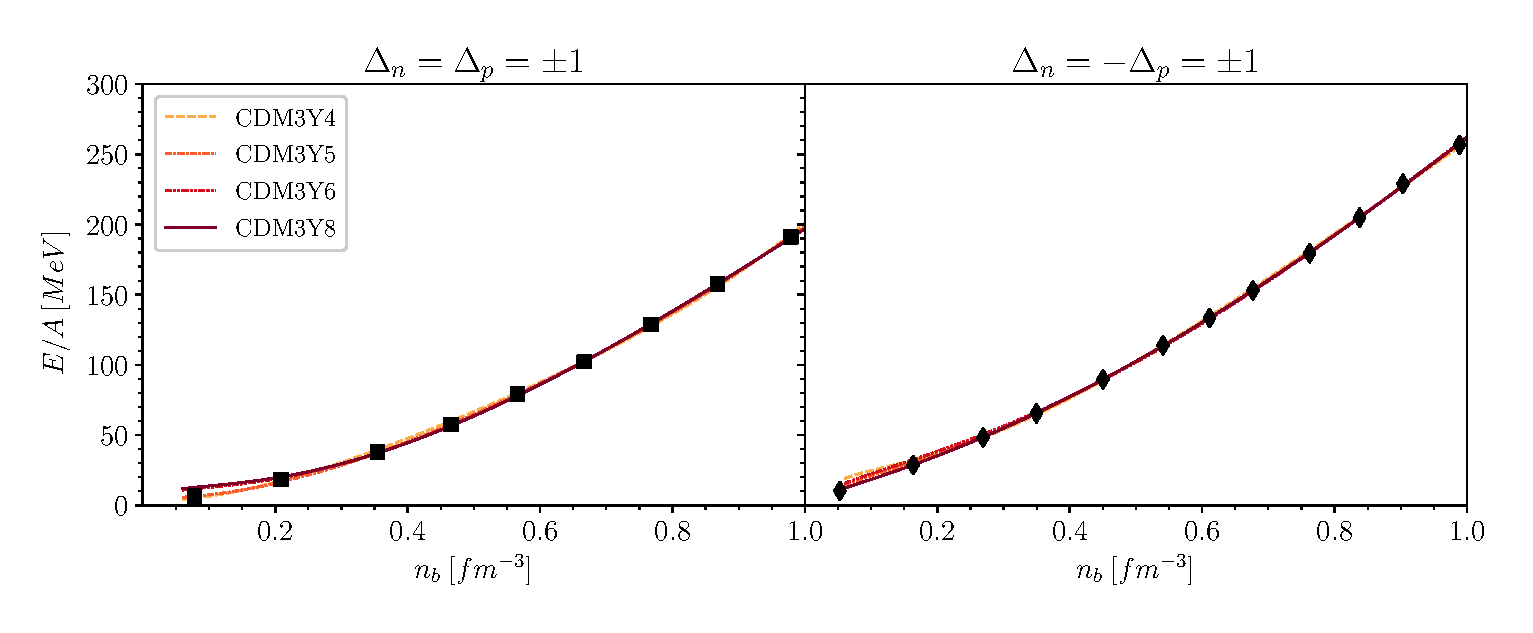
\includegraphics[width=\textwidth]{fig/BHF_fit.eps}
        \caption{Energy per baryon $E/A$ of symmetric \gls{NM} by the 5 CDM3Y$n$ and BDM3Y1 models compared to \gls{BHF} result \citep{vidana2002equation}. The diamond and square represent the \gls{BHF} result for $\Delta_n=-\Delta_p=\pm 1$ and $\Delta_n=\Delta_p=\pm 1$ respectively with $\Delta_\tau$ being the baryon spin polarization.}
        \label{fig:bhf}
\end{figure} 

\begin{table}[ht]
        \centering
        \caption{CDM3Y$n$ and BDM3Y1 interaction's parameters; the 00 and 01 terms are inherited from \citep{tan2021equation}, while the 10 and 11 parameters are added by fitting with \gls{BHF} result and $K$ is the incompressibility \eqref{eq:K} of spin-saturated symmetric \gls{NM} at saturation density $n_0\approx 0.17\:fm^{-3}$.}
        \label{tab:cd}
        \begin{tabular}{|C|C|C|C|C|C|C|}
                \hline
                \text{Interaction} & \sigma\tau & C_{\sigma\tau} & \alpha_{\sigma\tau} & \beta_{\sigma\tau} & \gamma_{\sigma\tau} & K\\
                                   & & & & (fm^3) & (fm^3) & (MeV)\\
                \hline
                \multirow{4}{*}{\text{CDM3Y3}} & 00 & 0.2985 & 3.4528 & 2.6388 & -1.5 &\multirow{4}{*}{217}\\
                                               & 01 & 0.2343 & 5.3336 & 6.4738 & 4.3172 &\\
                                               & 10 & 0.3890 & 3.5635 & -2.6717 & 20.3624 &\\
                                               & 11 & 0.8802 & 4.0433 & 12.3262 & 0.3662 &\\
                \hline
                \multirow{4}{*}{\text{CDM3Y4}} & 00 & 0.3052 & 3.2998 & 2.3180 & -2.0 &\multirow{4}{*}{228}\\
                                               & 01 & 0.2129 & 6.3581 & 7.0584 & 5.6091 &\\
                                               & 10 & 0.2593 & 6.0016 & -2.3377 & 18.8725 &\\
                                               & 11 & 0.8329 & 3.5941 & 9.2012 & 0.2690 &\\
                \hline
                \multirow{4}{*}{\text{CDM3Y5}} & 00 & 0.2728 & 3.7367 & 1.8294 & -3.0 &\multirow{4}{*}{241}\\
                                               & 01 & 0.2204 & 6.6146 & 7.9910 & 6.0040 &\\
                                               & 10 & 0.4106 & 5.6265 & -1.6698 & -1.9866 &\\
                                               & 11 & 0.6815 & 2.5833 & 5.1700 & 0.2578 &\\
                \hline
                \multirow{4}{*}{\text{CDM3Y6}} & 00 & 0.2658 & 3.8033 & 1.4099 & -4.0 &\multirow{4}{*}{252}\\
                                               & 01 & 0.2313 & 6.6865 & 8.6775 & 6.0182 &\\
                                               & 10 & 0.5186 & 9.9402 & 1.6698 & 2.9799 &\\
                                               & 11 & 0.6058 & 3.1947 & 4.4512 & 0.0822 &\\
                \hline
                \multirow{4}{*}{\text{CDM3Y8}} & 00 & 0.2658 & 3.8033 & 1.4099 & -4.3 &\multirow{4}{*}{257}\\
                                               & 01 & 0.2643 & 6.3836 & 9.8950 & 5.4249 &\\
                                               & 10 & 0.5997 & 9.1900 & 0.7514 & -4.7181 &\\
                                               & 11 & 0.3786 & 3.9435 & 2.7012 & 0.3512 &\\
                \hline
                \multirow{4}{*}{\text{BDM3Y1}} & 00 & 1.2521 & 0.0 & 0.0 & -1.7452 &\multirow{4}{*}{270}\\
                                               & 01 & 0.2528 & 7.6996 & 11.0386 & 6.3568 &\\
                                               & 10 & -1.3226 & -8.2559 & 0.0 & 17.2307 &\\
                                               & 11 & 0.1654 & 9.7394 & 1.6714 & -1.4893 &\\
                \hline
        \end{tabular}
\end{table}

\section{Equation of States of Nuclear Matter}%
\label{sec:equation_of_states_of_nuclear_matter}

In \gls{HF} formalism, the total \gls{HF} energy of the system can be expressed as
\begin{IEEEeqnarray*}{rCl}
        E_{HF} &=& \sum^{}_{\sigma\tau} \sum^{k_F^{\sigma\tau}}_{\bm{k}} \frac{\hbar^2 k^2}{2m_\tau} + \frac{1}{2} \sum^{}_{\bm{k}\sigma\tau} \sum^{}_{\bm{k'}\sigma'\tau'} \left[ \mel**{\bm{k}\sigma\tau,\bm{k'}\sigma'\tau'}{v^D}{\bm{k}\sigma\tau,\bm{k'}\sigma'\tau'} \right.\\
          && \left. \negmedspace{} + \mel**{\bm{k}\sigma\tau,\bm{k'}\sigma'\tau'}{v^{EX}}{\bm{k'}\sigma\tau,\bm{k}\sigma'\tau'} \right]\IEEEyesnumber
          \label{eqE}
\end{IEEEeqnarray*}  
where the single-particle wave function is plane wave
\begin{equation}
        \ket{\bm{k}\sigma\tau} = \frac{e^{i\bm{k}\cdot\bm{r}}}{ \sqrt{ \Omega}  } \chi_\sigma \chi_\tau
\end{equation}
with $\Omega$ being the spatial volume of the system, $k_F^{\sigma\tau} = (6\pi^2 n_{\sigma\tau})^{1/3}$ is the Fermi momentum corresponding to spin $\sigma$ and isospin $\tau$, $v^{D(EX)}$ is the direct (exchange) part of the interaction determined from the singlet and triplet-even (odd) of the central \gls{NN} force. Adopting the same functional form of \eqref{eq2-11}, the direct and exchange interaction is written as
\begin{IEEEeqnarray*}{rCl}
        v^{D(EX)}(n_b,r) &=& F_{00}(n_b) v^{D(EX)}_{00}(r) + F_{10}(n_b) v^{D(EX)}_{10}(r) \bm{\sigma}\cdot\bm{\sigma'}\\
                          &&\negmedspace{}+ F_{01}(n_b) v^{D(EX)}_{01}(r) \bm{\tau}\cdot\bm{\tau'} + F_{11}(n_b) v^{D(EX)}_{11}(r) (\bm{\sigma}\cdot\bm{\sigma'})(\bm{\tau}\cdot\bm{\tau'})\IEEEyesnumber
                          \label{eqHF}
\end{IEEEeqnarray*}
and
\begin{IEEEeqnarray*}{rCl}
        v^{D(EX)}_{\sigma\tau}(r) &=& \sum^{3}_{k=1} Y^{D(EX)}_{\sigma\tau}(k) \frac{\exp(-\mu_k r)}{\mu_k r} \IEEEyesnumber
\end{IEEEeqnarray*}  
with the Yukawa strengths given in Table \ref{tab:yukawa} and the density-dependent form factor parameters are in Table \ref{tab:cd}. Note that in \eqref{eqHF}, $n_b$ denotes the \emph{baryon density}, this will be used in order to distinguish with the lepton density in the later section.

\begin{table}[H]
        \centering
        \caption{Yukawa strengths of the M3Y-Paris interaction \citep{tan2020spin,anantaraman1983effective}.}
        \label{tab:yukawa}
        \begin{tabular}{|C|C|C|C|C|C|}
                \hline
                k & \mu_k & Y^D_{00} & Y^D_{10} & Y^D_{01} & Y^D_{11}\\
                    & (fm^{-1}) & (MeV) & (MeV) & (MeV) & (MeV)\\
                \hline
                1 & 4.0& 11061.625 & 938.875 & 313.625 & -969.125\\
                2 & 2.5 & -2537.5 & -36.0 & 223.5 & 450.0 \\
                3 & 0.7072 & 0.0 & 0.0 & 0.0 & 3.4877\\
                \hline\hline
                k & \mu_k & Y^{EX}_{00} & Y^{EX}_{10} & Y^{EX}_{01} & Y^{EX}_{11}\\
                    & (fm^{-1}) & (MeV) & (MeV) & (MeV) & (MeV)\\
                \hline
                1 & 4.0 & -1524.25 & -3492.75 & -4118.0 & -2210.0\\
                2 & 2.5 & -518.75 & 795.25 & 1054.75 & 568.75\\
                3 & 0.7072 & -7.8474 & 2.6157 & 2.6157 & -0.8719\\
                \hline
        \end{tabular}
\end{table}
Multiply \eqref{eqE} with $\Omega^{-1}$, the energy density of the \gls{NM} is separated into the kinetic term $\varepsilon_{kin}$ and the potential terms $\varepsilon_{\sigma\tau}$, i.e.
\begin{equation}
        \varepsilon_{HF} = \frac{E_{HF}}{\Omega} = \varepsilon_{kin} + F_{00}(n_b) \varepsilon_{00} + F_{01}(n_b) \varepsilon_{01} + F_{10}(n_b) \varepsilon_{10} + F_{11}(n_b) \varepsilon_{11}
\end{equation}
The final expressions of each terms of the energy density are
\begin{IEEEeqnarray}{rCl}
        \varepsilon_{kin} &=& \frac{3}{10} \sum^{}_{\sigma\tau} \frac{\hbar^2 (k_F^{\sigma\tau})^2}{m_\tau} n_{\sigma\tau}\\
        \varepsilon_{00} &=& \frac{1}{2} \left[ n_b^2 J^D_{00} + \int {A^2_{00} v^{EX}_{00}(r)} \: d^3 r \right] \\
        \varepsilon_{10} &=& \frac{1}{2} \left[ n_b^2 J^D_{10} \left( \Delta_n \frac{1+\delta}{2} + \Delta_p \frac{1-\delta}{2} \right)^2 + \int {A^2_{10} v^{EX}_{10}(r)} \: d^3 r \right] \\
        \varepsilon_{01} &=& \frac{1}{2} \left[ n_b^2 J^D_{01}\delta^2 + \int {A^2_{01} v^{EX}_{01}(r)} \: d^3 r \right] \\
        \varepsilon_{11} &=& \frac{1}{2} \left[ n_b^2 J^D_{11} \left( \Delta_n \frac{1+\delta}{2} - \Delta_p \frac{1-\delta}{2} \right)^2 + \int {A^2_{11} v^{EX}_{11}(r)} \: d^3 r \right]
\end{IEEEeqnarray}  
where $\Delta_{\tau} = (n_{\uparrow \tau} - n_{\downarrow \tau})/n_{\tau}$ is the polarization of nucleon, $\delta = (n_n - n_p)/n_b$ is the asymmetry of \gls{NM}, $J^D_{\sigma\tau} = \int v^D_{\sigma\tau}(r)\: d^3 r$ is the volume integral of the direct interaction and
\begin{equation}
        \begin{array}{l}
                A_{00} = n_{\uparrow n} \hat{j_1}(k_F^{\uparrow n} r) + n_{\downarrow n} \hat{j_1}(k_F^{\downarrow n} r) + n_{\uparrow p} \hat{j_1}(k_F^{\uparrow p} r) + n_{\downarrow p} \hat{j_1}(k_F^{\downarrow p} r)\\[5pt]
                A_{10} = n_{\uparrow n} \hat{j_1}(k_F^{\uparrow n} r) - n_{\downarrow n} \hat{j_1}(k_F^{\downarrow n} r) + n_{\uparrow p} \hat{j_1}(k_F^{\uparrow p} r) - n_{\downarrow p} \hat{j_1}(k_F^{\downarrow p} r)\\[5pt]
                A_{01} = n_{\uparrow n} \hat{j_1}(k_F^{\uparrow n} r) + n_{\downarrow n} \hat{j_1}(k_F^{\downarrow n} r) - n_{\uparrow p} \hat{j_1}(k_F^{\uparrow p} r) - n_{\downarrow p} \hat{j_1}(k_F^{\downarrow p} r)\\[5pt]
                A_{11} = n_{\uparrow n} \hat{j_1}(k_F^{\uparrow n} r) - n_{\downarrow n} \hat{j_1}(k_F^{\downarrow n} r) - n_{\uparrow p} \hat{j_1}(k_F^{\uparrow p} r) + n_{\downarrow p} \hat{j_1}(k_F^{\downarrow p} r)
        \end{array}
\end{equation}
with $\hat{j}_1(x)=3j_1(x)/x$ and $j_1(x)$ being the 1\textsuperscript{st} order spherical Bessel function.\par
In the parabolic approximation \citep{khoa1996study}, the energy density per nucleon $E/A$ can also be expanded in terms of the asymmetry $\delta$ as
\begin{equation}
    \frac{E}{A} (n_b, \delta, \Delta_n, \Delta_p) = \frac{\varepsilon_{HF}}{n_b} = \frac{E}{A} (n_b, \delta=0, \Delta_n, \Delta_p) + S(n_b, \Delta_n, \Delta_p)\delta^2 + \mathcal{O}(\delta^4)
    \label{eq:S}
\end{equation}
with $S$ being the \emph{nuclear symmetry energy}. The symmetry coefficient $J$, slope parameter $L$ and curvature $K_{sym}$ are taken by expanding the symmetry energy at saturation density $n_0$, i.e. \citep{tan2020spin,li2008recent,horowitz2014way,lattimer2014symmetry}
\begin{equation}
    S(n_b, \Delta_n, \Delta_p) = J(\Delta_n, \Delta_p) + \frac{L(\Delta_n, \Delta_p)}{3} \left( \frac{n_b - n_0}{n_0} \right) + \frac{K_{sym}(\Delta_n, \Delta_p)}{18} \left( \frac{n_b - n_0}{n_0} \right)^2 + \ldots
    \label{eq:pars}
\end{equation}
along with the nuclear incompressibility at saturation density
\begin{equation}
    K(\Delta_n, \Delta_p) = 9 \left.\pdv{P(n_b, \delta=0,\Delta_n,\Delta_p)}{n_b}\right|_{n_b \to n_0}
        \label{eq:K}
\end{equation}
These are the quantity that will be used in order to compared with the empirical values in Chapter \ref{chap:result}.

\section{\textbeta-Stable Nuclear Matter}%
\label{sec:textbeta_stable_nuclear_matter}

After the \gls{HF} calculation, we were able to obtain a numerical \gls{HF} energy density $\varepsilon_{HF}$. However, it is in fact impossible for a \gls{NS} to exist while consisting of purely nucleon. In order to compensate for this issue, leptons ($e^-$ and $\mu^-$) have to be introduced to the matter constituents and the $npe\mu$ matter has to satisfy the \emph{\textbeta-stable} condition \citep{glendenning2012compact}, i.e.
\begin{itemize}
        \item Charge balance
                \begin{equation}
                        n_p = n_e + n_\mu
                        \label{chargeEQ}
                \end{equation}
        \item Chemical potential balance
                \begin{equation}
                        \mu_n - \mu_p = \mu_e = \mu_\mu
                \end{equation}
                where $\mu_i = \pdv{\varepsilon}{n_i}$ ($i=n,p,e,\mu$) is the chemical potential of the $i$ particle.
\end{itemize}
The total energy density of the $npe\mu$ matter is thus
\begin{equation}
        \varepsilon = \varepsilon_{HF} + n_n m_n c^2 + n_p m_p c^2 + \varepsilon_e + \varepsilon_\mu 
\end{equation}
which leads to the nucleon chemical potential of the form
\begin{equation}
        \mu_\tau (n_n,n_p,\Delta_n,\Delta_p) = \frac{\partial \varepsilon}{\partial n_\tau}  = \frac{\partial \varepsilon_{HF}}{\partial n_\tau} + m_\tau c^2
\end{equation}
Let $\hat{\mu} = \mu_n - \mu_p$ be the leptons' chemical potential, \eqref{chargeEQ} is equivalent to\footnote{$\theta(x)$ is the Heaviside function, i.e. it returns $1$ for $x\geq 0$ and $0$ otherwise.}
\begin{equation}
        3\pi^2 (\hbar c)^3 n_p - \hat{\mu}^3 - \left[ \hat{\mu}^2 - (m_\mu c^2)^2 \right]^{3/2} \theta(\hat{\mu} - m_\mu c^2) = 0
\end{equation}
from which the proton fraction $x_p = n_p/n_b$ can be obtained as shown in Figure \ref{fig:xp}, note that only beyond the muon threshold density $\mu_e > m_\mu c^2 \approx 105.6\:MeV$ do muons appear in the system. Furthermore, under strong magnetic field like that of a magnetar, we can approximate $\Delta_n \approx -\Delta_p \approx \Delta$ and reduce the \gls{EoS} to depend on just the baryon polarization $\Delta$ alone, and the more baryon polarized, the stronger the magnetic field of the \gls{NS}.\par
For a fixed value of $\Delta$, we are able to obtain a density function of the form $n_n (n_b, \Delta)$ and $n_p (n_b, \Delta)$, which in turn gives the lepton chemical potential $\hat{\mu}(n_b,\Delta) = \hat{\mu}(n_n,n_p)$ On the other hand, the leptons' densities are then \citep{loan2011equation}
\begin{equation}
        n_e(n_b,\Delta) = \frac{ \hat{\mu}^3(n_b,\Delta)}{ 3\pi^2 (\hbar c)^3} \quad\text{and}\quad n_\mu(n_b,\Delta) = \frac{ \Big[\hat{\mu}^2(n_b,\Delta) - (m_\mu c^2)^2\Big]^{3/2}}{ 3\pi^2 (\hbar c)^3} \theta(\hat{\mu}(n_b,\Delta)-m_\mu c^2)
\end{equation} 
Consider the $e^-$ and $\mu^-$ to be systems of relativistic Fermi gas, then their respective energy densities and pressure contributions are ($l=e,\mu$) \citep{moustakidis2009equation}
\begin{equation}
        \varepsilon_l(n_b,\Delta) = \frac{ 2}{ (2\pi)^3} \int_{{0}}^{{[3\pi^2n_l(n_b,\Delta)]^{1/3}}} {\sqrt{\hbar^2 c^2 k^2 + m_l^2 c^4}} \: d^3{\mathbf{k}}
\end{equation} 
and
\begin{equation}
        P_l(n_b,\Delta) = \frac{ 1}{ 3} \frac{ 2}{ (2\pi)^3} \int_{{0}}^{{[3\pi^2 n_l(n_b,\Delta)]^{1/3}}} { \frac{ \hbar^2 c^2 k^2}{ \sqrt{\hbar^2 c^2 k^2 + m_l^2 c^4}} } \: d^3{\mathbf{k}}
\end{equation} 
Plus, from the \gls{HF} formalism with \gls{NM}, the baryon pressure is given by
\begin{equation}
        P_b = n_b^2 \pdv{(\varepsilon_{HF}/n_b)}{n_b}
\end{equation}
Finally, we obtain the total energy density-dependence on baryon density as 
\begin{equation}
        \varepsilon(n_b,\Delta) = \varepsilon_{HF}(n_b,\Delta) + n_n(n_b,\Delta)m_n c^2 + n_p(n_b,\Delta)m_p c^2 + \varepsilon_e(n_b,\Delta) + \varepsilon_\mu(n_b,\Delta)
\end{equation}
and the total pressure of \gls{NS} matter
\begin{equation}
        P(n_b,\Delta) = P_b(n_b,\Delta) + P_e(n_b,\Delta) + P_\mu(n_b,\Delta)
\end{equation}
In addition, the \gls{EoS} of the \gls{NS}'s crust (low baryon density region) is adopted from the Compress Liquid Drop Model calculation \citep{douchin2000nuclear,douchin2001unified}. The complete \gls{EoS} of cold $\beta$-stable \gls{NS} matter is later discussed in Chapter \ref{chap:result}.

\section{Density dependence of the spin polarization}%
\label{sec:density_dependence_of_the_spin_polarization}

In the above calculation, the baryon spin polarization $\Delta$ was taken to be independent of the baryon density $n_b$; however, due to the complexity of the magnetic field distribution inside the \gls{NS} \citep{fujisawa2014magnetic}, this does not fully reflect the reality. Particularly, in the inner core of the \gls{NS}, baryons are heavily compressed at extremely high density by gravity, which leads to the full degeneracy, i.e. all possible quantum states are occupied, of baryons in this region and there is no room for baryon to change its spin orientation. Along with the magnetic field, the spin polarization of baryon is expected to gradually weaken to $\Delta \approx 0$ the nearer to the \gls{NS} center, in other words, at higher density \citep{fujisawa2014magnetic,tan2020spin}. Although it's beyond the scope of the current study to accurately calculate the density-dependence of $\Delta(n_b)$, we will explore such effect by investigating different scenarios proposed by \cite{tan2020spin} based on the magnetic field distribution of magnetar obtained by \cite{fujisawa2014magnetic}, i.e.
\begin{enumerate}[label=(\Alph*)]
    \item The magnetic field is strongly localized in the surface region of the \gls{NS}, near the crust-core transition, and falls to $B\approx 0$ at $n_b \approx 0.18\: fm^{-3}$,
    \item The magnetic field distribution is broader and decreases gradually to zero at a denser region, which cover both the crust and the outer core, of $n_b \approx 0.35\:fm^{-3}$.
\end{enumerate}
Each scenario was considered with $\Delta_0 = \Delta(n_b \approx 0)$ at the value of partial polarization $\Delta_0 = 0.6$, $0.8$ and total polarization $\Delta_0 = 1.0$ as shown in Figure \ref{fig:Delta}
\begin{figure}[ht!]
    \centering
    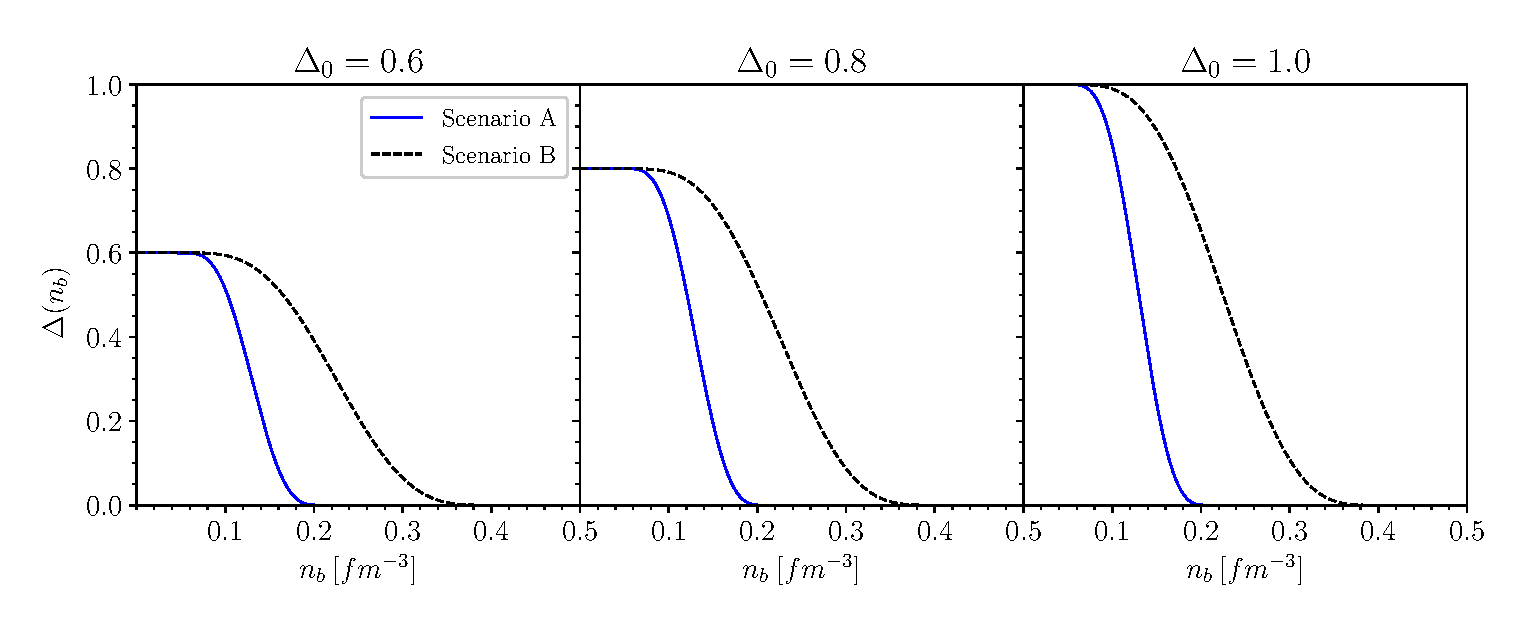
\includegraphics[width=\textwidth]{fig/Delta.eps}
    \caption{Scenarios of the density-dependence of the baryon spin polarization at 3 levels of $\Delta_0$.}
    \label{fig:Delta}
\end{figure} 
